\cleardoublepage
\phantomsection
\chapter*{Introduction}
 
The audio-visual media content production industry (e.g.: broadcasters, small production companies, \ldots) has been, and already is, employing rigid and difficult to scale technologies to transport and manage their streams through their processing chain. But, since early 2000s, a gradually adoption of IP technologies has been happening. Key examples of this adoption are that TV content media production is already digital based (i.e.: broadcasting channels) and its media transport layer is circuit oriented. Moreover, IP networks offer enhancements over operational and cost issues and it is the next step to the audiovisual media production.

Since few years ago, the broadcasting industry is pushing on to adopt IP as the transport technology because of several benefits such as:

\begin{itemize}
  \item Enhanced agility and flexibility of the broadcast workflows
  \item Convergence of services (i.e.: audio, video, metadata and generic data)
  \item Format agnosticism to support the adoption of coming new UHDTV formats such as 8K 
  \item Economy of scale by integrating broadcasting industry into the far more massive IT industry
\end{itemize}

But there is still a lot of work to be done to achieve complete IP convergence, and lots of new possibilities thanks to different architectures and configurations that can be applied on OTT (Over-The-Top \cite{ottVSiptv}) content management systems. 

Despite almost all post-production environments has become file-based they can now be completely migrated to IP infrastructures. Main examples are some control and management services, and media content distribution over Internet (i.e.: live or on demmand media streaming to end-users) or over proprietary networks (i.e.: IPTV \cite{ottVSiptv}).

Nevertheless, the live production environment has yet to be migrated to IP. Main reasons are due to some stringent constraints such as levels of synchronization, extremely low packet loss levels, high-bandwidth demand or jitter variation, because these are not all intrinsically assured by current IP technologies.

Figure \ref{F:bebooss} helps understanding where this thesis is focusing and what is its goal:  to offer specific solutions and tools for real-time media content production over cloud infrastructures. Therefore, this thesis is mainly focused on the "Live production" step of figure \ref{F:bebooss}, where related participants (i.e.: people, cams, mixers, ...) are aimed to be networked or moved to an IP and virtualized environment.

\begin{figure}[!htb]
\begin{center}
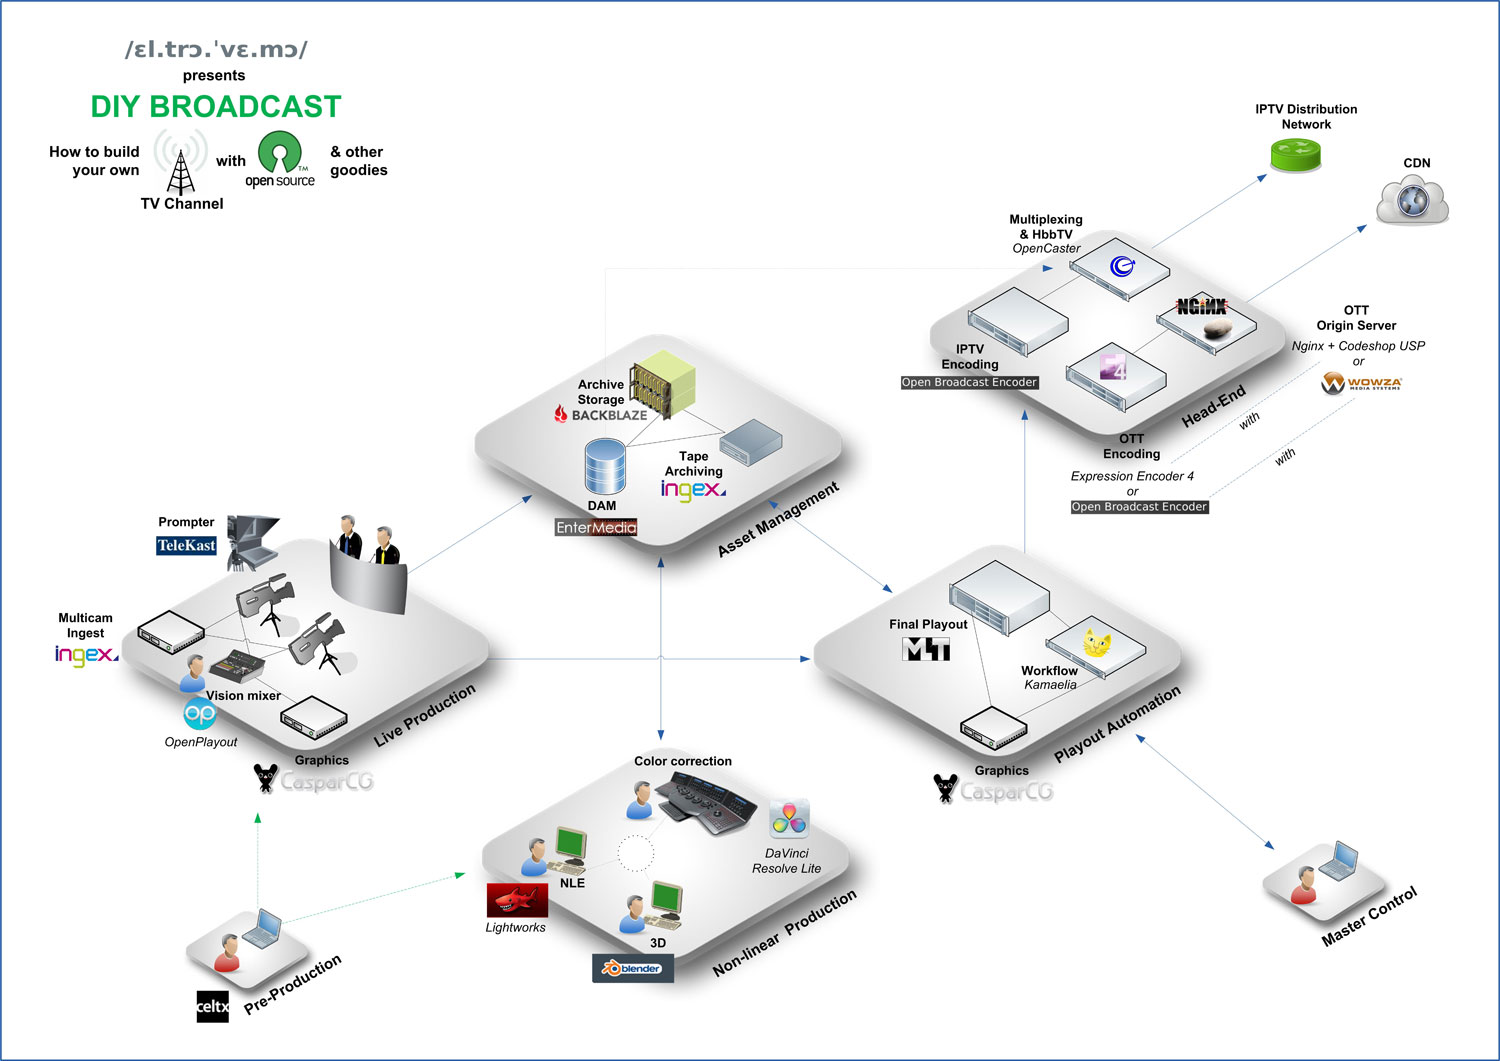
\includegraphics[width=1\textwidth]{./images/DIY_broadcast_platform_exportweb.jpg}
\caption{Broadcasting example based on open-source softwares \cite{bexample}}
\label{F:bebooss}
\end{center}
\end{figure}

Then, next topics are going to be studied together with the aim to propose and develop a platform prototype. Moreover, this platform prototype will be deployed in an experimental environment in order to demonstrate and validate the proposal. 

\begin{itemize}
\item Virtualization layer \hfill 

The virtualization paradigm offers specific solutions to improve scalability, robustness and reliability of any platform and services to be deployed over a cloud environment (n-tier applications development \cite{n-tier architecture}). 

\item Monitoring layer \hfill 

The monitoring layer is a crucial system tool to be deployed which offers the capability of getting non-stop feedback from deployed services in order to actuate in real-time over any defined alarm. This layer gives also the chance to find and solve infrastructure/platform bottle-necks.

\item Application layer \hfill 

The application layer is the core service itself (the audio and video production core service) that must be adapted in order to offer full compatibility with previous mentioned layers and to become a cloud service.

\end{itemize}

All the items above-mentioned are related to this thesis execution period that is aligned with specific goals of the i2CAT Foundation Audiovisual Unit \cite{i2catua}, which has specific research challenges such as to study and propose enhancements for networked media and interactive and immersive media related topics. 

Specifically, this thesis is one of the next steps related to the LiveMediaStreamer framework project \cite{lmsGITHUB}, an open-source software developed in the Audiovisual Unit's technical team. One of this main functionalities is the capability of working as a software-based audio and video mixer, and this is the scenario that is going to be focused as the main service to be analysed.

Finally, this thesis is organized as follows: chapter \ref{A:stateOfTheArt} is about the state of the art of related technologies of the audiovisual content production, where the steps already done for convergence IP are briefly explained. Moreover, an introduction of the cloud concept and the topics related of this thesis are also shown. In chapter \ref{B:problemStatementAndProposal}, the problem statement are presented with a proposal solution, which are based on the topics already explained. Then, chapter \ref{D:application} (application), \ref{D:virtualization} (virtualization) and \ref{G:monitoringLayer} (monitoring) are each one focused on how the proposal solutions are developed. Then, in chapter \ref{H:platformDeploymentAndDemonstrations}
, specific deployments and demonstrations of the solutions proposed are carried out. And, last chapter \ref{C:conclusions} is showing the conclusions obtained of the overall thesis.





